\documentclass[tikz,border=0pt,11pt]{standalone}
\usepackage{amsmath, amssymb}
\usetikzlibrary{
	3d, % For 3D drawing
	angles,
	arrows,
	arrows.meta,
	backgrounds,
	bending,
	calc,
	decorations.pathmorphing,
	decorations.pathreplacing,
	decorations.markings,
	fit,
	matrix,
	patterns,
	patterns.meta,
	positioning,
	shadows,
	shapes,
	shapes.geometric,
	tikzmark,
	quotes
}
\usepackage[T1]{fontenc}
\usepackage[utf8]{inputenc}
\usepackage{newpxtext,newpxmath}
\usepackage{sectsty}

\definecolor{accent}{HTML}{1F4E79}
\definecolor{softaccent}{HTML}{EAF2F8}
\definecolor{softgray}{HTML}{F6F7F9}
\definecolor{successdraw}{HTML}{27AE60}
\definecolor{successfill}{HTML}{EAFAF1}
\definecolor{errordraw}{HTML}{C0392B}
\definecolor{errorfill}{HTML}{FDEDEC}
\newcommand{\F}{\mathbb{F}}

\begin{document}
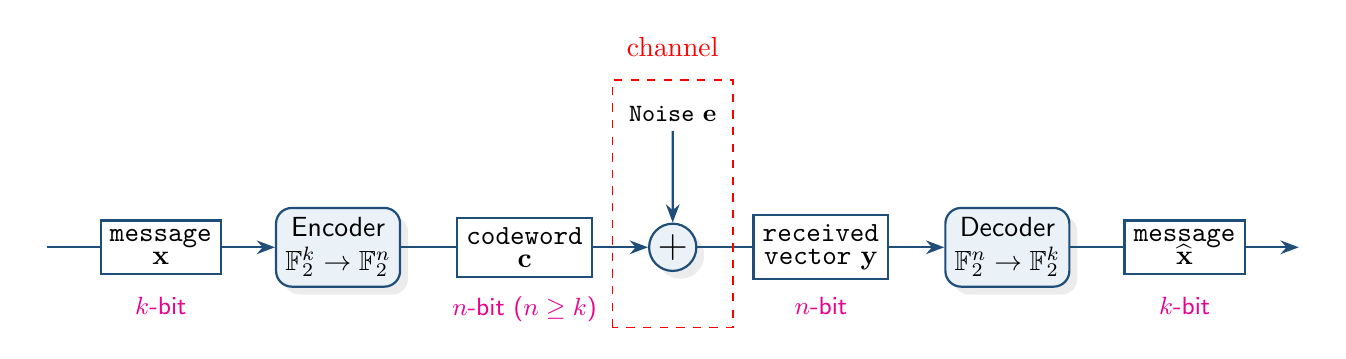
\begin{tikzpicture}[
	>=Stealth,
	block/.style={
		draw=accent, thick, fill=softaccent, rounded corners=2mm,
		minimum width=1.2cm, minimum height=1cm, align=center,
		font=\sffamily, drop shadow={opacity=0.15, shadow xshift=1mm, shadow yshift=-1mm}
	},
	adder/.style={
		circle, draw=accent, thick, fill=softaccent,
		minimum size=6mm, inner sep=0pt, align=center, font=\Large,
		drop shadow={opacity=0.15, shadow xshift=1mm, shadow yshift=-1mm}
	},
	arrow/.style={->, thick, accent},
	mathlabel/.style={font=\normalsize, text=black},
	sublabel/.style={font=\small\sffamily, text=magenta},
	scale=.85
	]
	
	% Invisible nodes to act as the start and end points of the signals
	\node (start) at (0,0) {};
	\node (end)   at (19,0) {};
	
	% Main operational blocks
	\node[block, align=center] (enc) at (4.5,0) {Encoder\\ $\F_2^k\to\F_2^n$};
	\node[adder] (add) at (9.5,0) {$+$};
	\node[block, align=center] (dec) at (14.5,0) {Decoder\\ $\F_2^n\to\F_2^k$};
	
	% Noise entry point
	\node (noise) at (9.5, 2) {\small \texttt{Noise} \textbf{e}};
	
	% --- Signal Paths & Labels ---
	
	% Source to Encoder
	\draw[arrow] (start) -- 
	node[midway, mathlabel, draw=accent, fill=white, align=center] {\texttt{message}\\ [-1.25mm] $\textbf{x}$} 
	node[below=5mm, sublabel] {$k$-bit} 
	(enc);
	
	% Encoder to Channel (Adder)
	% We use a standard label below the arrow to replace the underbrace in the equation
	\draw[arrow] (enc) -- 
	node[midway, mathlabel, draw=accent, fill=white, align=center] {\texttt{codeword}\\ [-1.25mm] $\textbf{c}$} 
	node[below=5mm, sublabel] {$n$-bit ($n \geq k$)} 
	(add);
	
	% Noise entering the Channel
	\draw[arrow] (noise) -- (add);
	
	% Channel to Decoder
	\draw[arrow] (add) -- 
	node[midway, mathlabel, draw=accent, fill=white, align=center] {\texttt{received}\\ [-1.25mm]  \texttt{vector} $\textbf{y}$} 
	node[below=5mm, sublabel] {$n$-bit} 
	(dec);
	
	% Decoder to Destination
	\draw[arrow] (dec) -- 
	node[midway, mathlabel, draw=accent, fill=white, align=center] {\texttt{message}\\ [-1.25mm] $\widehat{\textbf{x}}$} 
	node[below=5mm, sublabel] {$k$-bit} 
	(end);
	
	\draw[dashed, red] (8.6,-1.2) rectangle (10.4,2.5);
	\node[red] at (9.5,3) {channel};
\end{tikzpicture}
\end{document}